\documentclass[11pt,a4paper]{article}
\usepackage{amsmath}
\usepackage[utf8]{inputenc}
\usepackage{graphicx}	%Grafiken


\title{Abstract of Computer Graphics}
\author{Andreas Ruscheinski \ Christian Delfs}
\date{}
\begin{document}
\maketitle

\section{Introduction}
	\subsection{What is Computer Graphics?}
		\begin{itemize}
			\item deals with all aspect of image creation with computers
		\end{itemize}
	\subsection{Application Areas}
	\subsection{History}
	\subsection{Image formation}
		\begin{itemize}
			\item form images on a two dimensional device analogous how images are formed by physical systems (Cameras and so on)
			\item Objects, Viewer, Light sources with attributes how light interacts with materials in scene, IMPORTEND: independence of object, viewer and light sources
			\item Ray Tracing: follow rays from light with maybe collusions with object to lens (camera) or going to infinity
			\item Luminance Image: Monochromatic (grey levels) like black-white-films
			\item Color Image: perceptional attributes (hue, saturation, lightness)
			\item Additive Color: adding amouts of three primaries (RGB), Monitor
			\item Subtractive Color: form color by filter white light (CYM), Printing
			\item Pinhole Camera: use trigonometry to find project 
			\begin{center}
				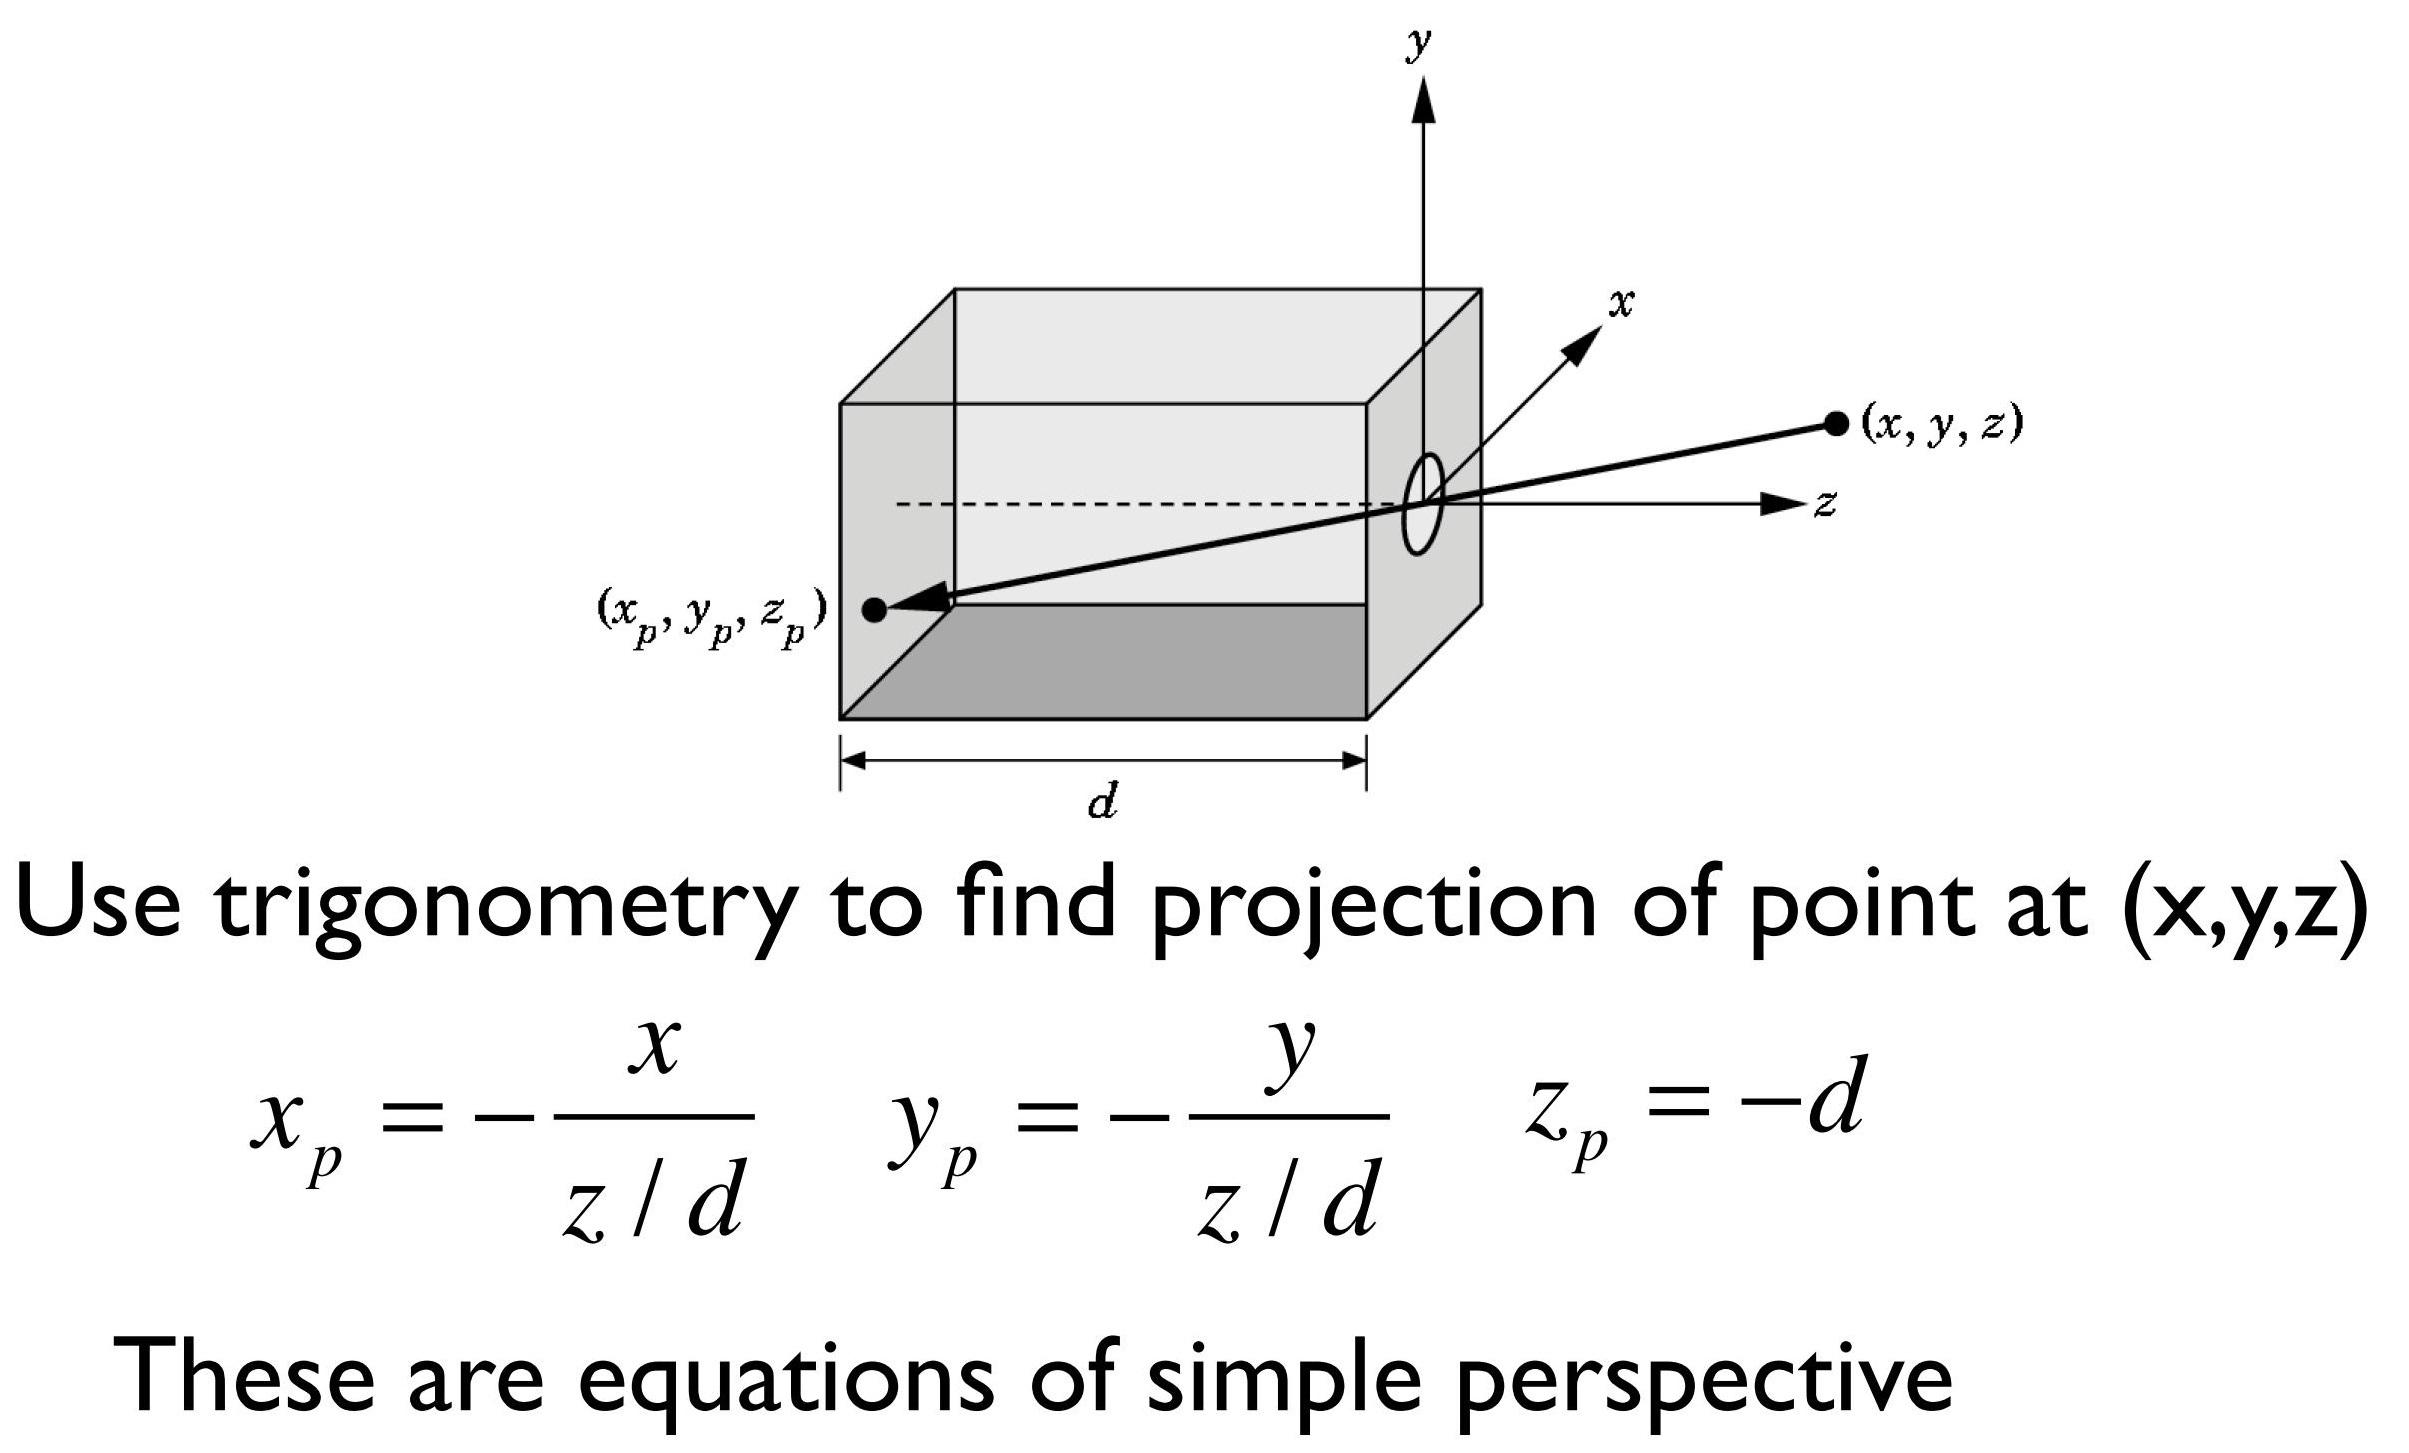
\includegraphics[scale=0.3]{pictures/pic1.jpg}
			\end{center}
			\item Synthetic Camera: projection of image on image plane, camera views on image plane ?????
			\item Advantages of SC: separation of objects, viewer, light sources, two-dimensional graphics is a special case of three-dimensional graphics, simple api with fast hardware implementation
			\item cant compute color or shade of each object independently reasons: blocked form light, reflects, translucent
			\item disadvantages of ray tracing: easy calculation for easy object, but on compley objects FUCK UP especially with lights and shadows
		\end{itemize}
	\subsection{Basic Architecture} 
		\begin{itemize}
			\item Physical Approaches: RayTracing = SLOW, can handle global effects; Radiosity: Energy based approaced = MUCH SLOWER
			\item Practical Approaches: process one object at time, can only handle local lightning, pipeline architecture
			\begin{center}
				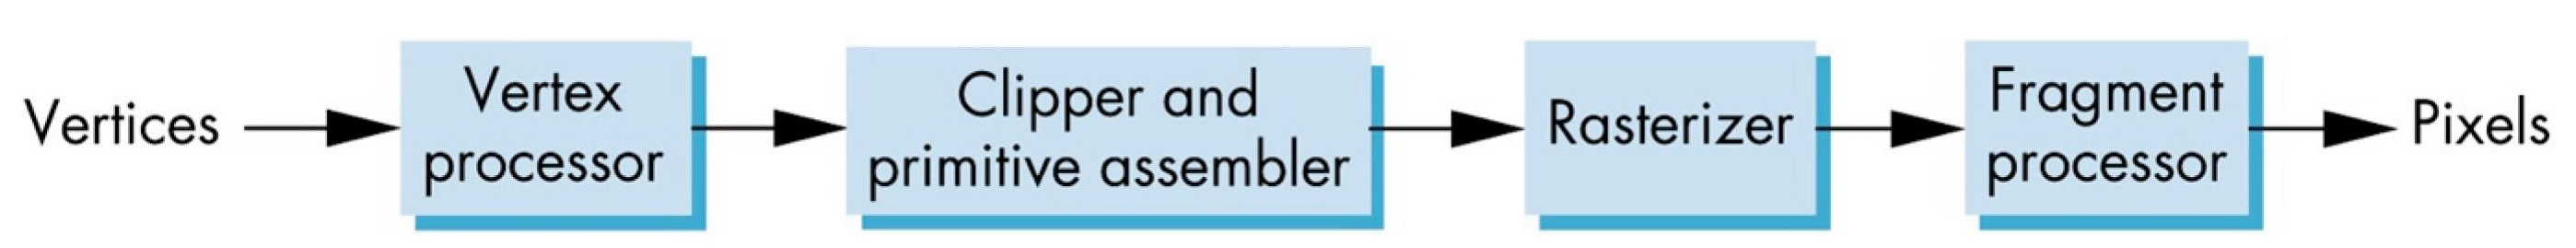
\includegraphics[scale=0.5]{pictures/pic4.jpg}
			\end{center}
			\item Vertex Processing: much work is converting object representations form one coordinate system to another (Object Coordinates, Camera Coordinates, Screen Coordinates)
			\begin{itemize}
				\item Projection: combines 3D viewer with the 3D objects to produce the 2D image
				\item Perspective Projection: all Projectors meet the center of projection
				\item Parallel Projection: projectors are parallel, center of projection is replaced by a direction of projection
			\end{itemize}
			\item Primitve Assembly: vertices must be collected into geometric objects (line segments, polygons, curves and surfaces)
			\begin{itemize}
				\item Clipping: a real camera cannot see the whole world, objects that are not within this volume are said to be clipped out of the scene
			\end{itemize}
			\item Rasterization: create fragments (potential pixels), fragments have locations in frame buffer, color and depth attributes, vertex attributes are interpolated over objects by the rasterizer
			\item Fragment Processing: fragments are processed to determinate the color of pixel in frame buffer, color determined by texture mapping or interpolation of vertex colors, fragments may blocked by other fragments coloser to camera (hidden surface removal)
			\item Programmiers Interface:
			\begin{itemize}
				\item API
				\item specifiy what we nee to form an image (objects, viewer, light sources, materials), handling input from devices
				\item Object Specification: limited set of primitives (points, line segments, polygons, some surfaces)
				\item Camera Specification: postion of center of lens, orientations, lens, film size, orientation of film plane
				\item Light: different types of lights (point lights, spot light, near and far sources, color properties)
				\item Material: absorption, diffuse, specular
			\end{itemize}
		\end{itemize}
	\subsection{RayTracing}
		\begin{itemize}
			\item follow rays of light from a point source
			\item Problems: rays do not affect what we see, scattering produces many rays; Better: ray casting
			\item Ray Casting: rays goes from view to scene, one ray for one pixel
			\item objects are build from primitives and set operations with other objects
			\item Ray is parametric, Sphere is quadric (quadric is a solution set of quadratic functions), Resulting equations is a entry/exit point or no solution if ray misses
			\item one point is visable if we hit light source form point
			\item in case of reflection follow rays from transmitting surfaces, recursive process
			\item Structure: recursivly, calculate for each ray, find intersection with closet surfaces (need object datebase, complexity of calculation limits of object types), compute lightnig at surface, trace reflected and transmittet rays
			\item stop of procedure if no track amout left (some light will be absorbed at each intersetion with object), ignore rays that go of to infinity (workaround, large absorbing sphere around problem), cout steps
			\item color of pixel is the result of local+reflected+transmitted
			\item Computing Intersections, solve equations with maybe nurmerical methods 
			\item easy calculation with planes
			\item polyhedra build from planes
			\item ray enters at furthest intersection with front facing plane, leaves at closest intersection with back facing planes,
			\item if entry is further away then exit,ray muss miss the polehedron
		\end{itemize}

\section{Basic OpenGL}
	\subsection{Architecture}
		\begin{itemize}
			\item  a platform-independent API (Easy to use,  Close enough to the hardware to get excellent performance)
			\item  Focus on rendering
			\item Relatively stable
			\item Evolution reflect new hardware capabilities (3D texture mapping and texture objects, Vertex programs)
			\item OpenGL Libraries
				\begin{itemize}
					\item OpenGL core library (OpenGL32 - Windows,  GL - most unix/linux systems (libGL.a))
					\item OpenGL Utility Library (GLU) (Provides functionality in OpenGL core but avoids having to rewrite code)
				\end{itemize}
			\item OpenGL Functions
				\begin{itemize}
					\item Primitives (Points, Line Segments, Polygons)
					\item Attributes
					\item Transformations (Viewing, Modeling)
					\item Control (GLUT)
					\item  Input (GLUT)
					\item Query
				\end{itemize}
			\item OpenGL Architecture
			\begin{center}
				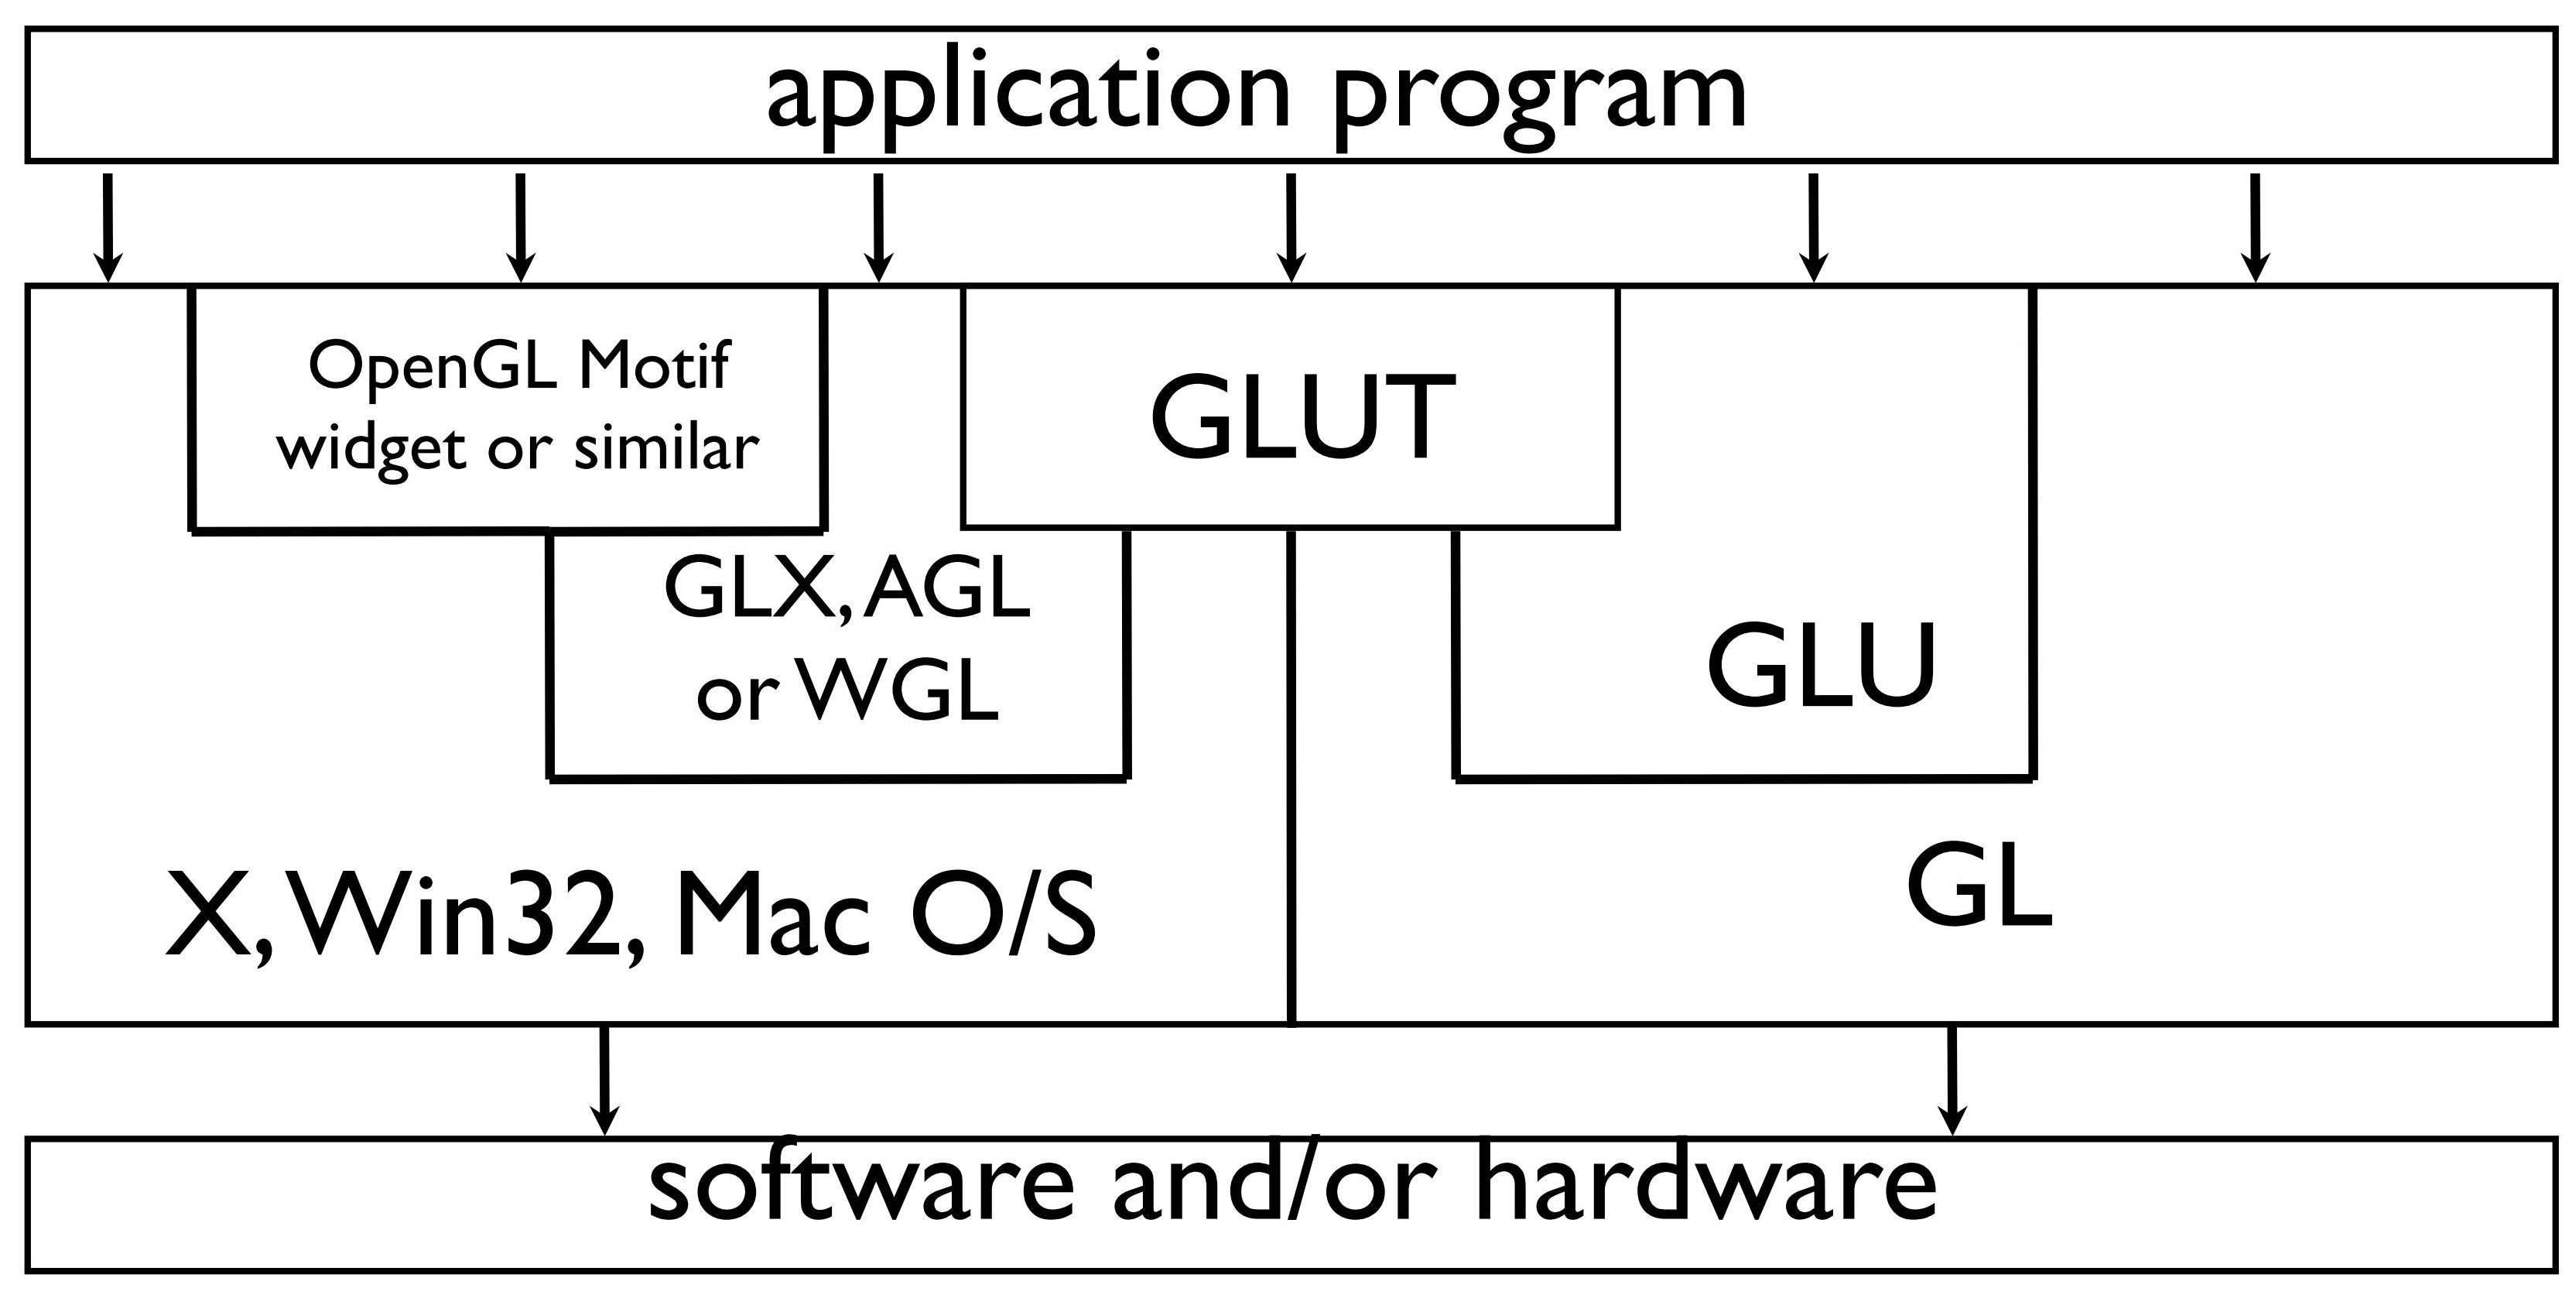
\includegraphics[scale=0.3]{pictures/pic2.jpg}
			\end{center}
			\item Software Organization
			\begin{center}
				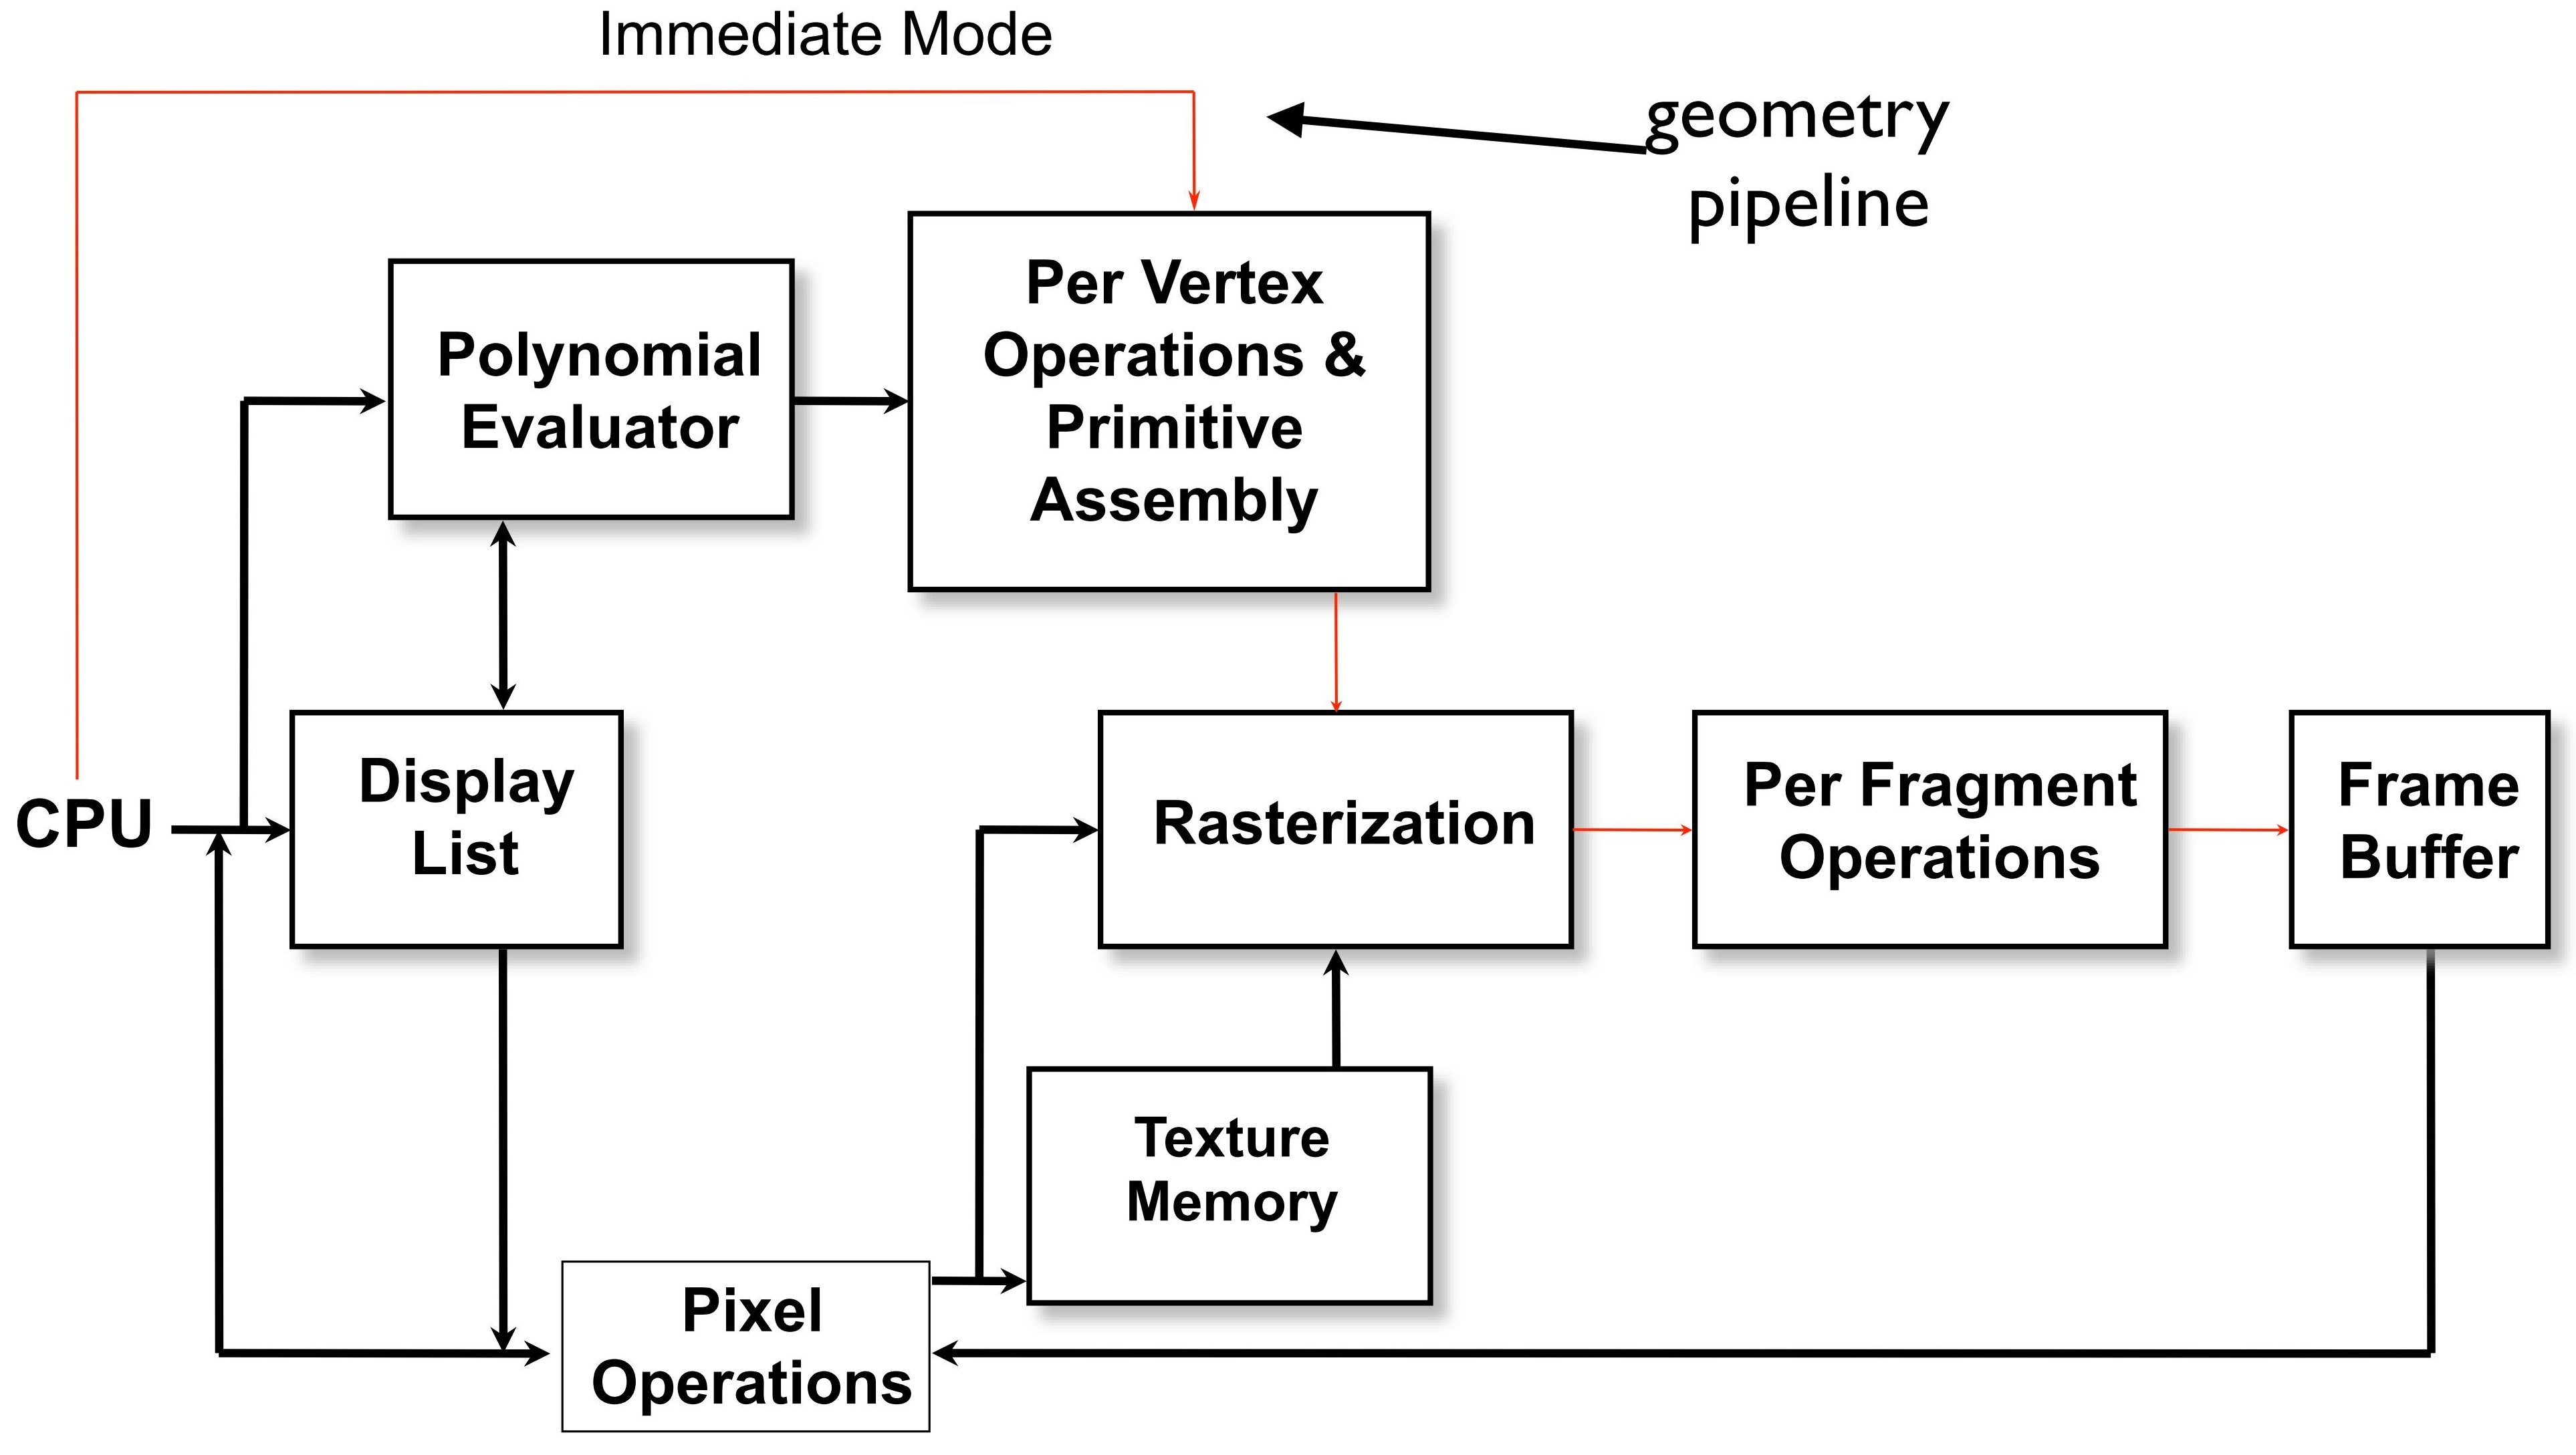
\includegraphics[scale=0.3]{pictures/pic3.jpg}
			\end{center}
			\item OpenGL is a state machine
			\item OpenGL functions are of two types
				\begin{enumerate}
					\item Primitive generating \\
						(Can cause output if primitive is visible, How vertices are processed and appearance of primitive are controlled by the state)
					\item State changing\\
						(Transformation functions, Attribute functions)
				\end{enumerate}
			\item OpenGL is not object oriented so that there are multiple functions for a given logical function (glVertex3f, glVertex2i, glVertex3dv)
		\end{itemize}
	\subsection{GLUT - OpenGL Utility Toolkit}
		\begin{itemize}
			\item  Provides functionality (Open a window, Get input from mouse and keyboard, Menus, Event-driven)
			\item GLUT function
				\begin{description}
					\item[glutInit] allows application to get command line arguments and initializes system
					\item[gluInitDisplayMode] requests properties for the window (the rendering context) 	
					\item[glutWindowSize] in pixels
					\item[glutWindowPosition] from top-left corner of display 	
					\item[glutCreateWindow] create window with title “simple” 	
					\item[glutDisplayFunc] display callback
					\item[glutMainLoop] enter infinite event loop						
				\end{description}
		\end{itemize}
	\subsection{Simple programs in two and three dimensions}
		\begin{itemize}
			\item  Event Loop
			\begin{itemize}
				\item Note that the program defines a display callback function named mydisplay
				\item Every glut program must have a display callback
				\item The display callback is executed whenever OpenGL decides the display must be refreshed, for example when the window is opened
				\item The main function ends with the program entering an event loop
			\end{itemize}
			\item Objectives
			\item Program Structure \\
				(Most OpenGL programs have a similar structure that consists of	the following functions)
				\begin{itemize}
					\item \textbf{main():} defines the callback functions; opens one or more windows with the required properties; enters event loop (last executable statement)	
					\item \textbf{init():} sets the state variables	(Viewing, Attributes)
					\item \textbf{callbacks:} Display function, Input and window functions
				\end{itemize}
			\item TODO: 06-5 PIC
			\item Coordinate Systems
				\begin{itemize}
					\item The units in glVertex are determined by the application and are called object or problem coordinates	
					\item The viewing specifications are also in object	coordinates and it is the size of the viewing volume that determines what will appear in the image	
					\item Internally, OpenGL will convert to camera (eye) coordinates and later to screen coordinates 	
					\item OpenGL also uses some internal representations that usually are not visible to the application
				\end{itemize}
			\item OpenGL Camera TODO: 06-10 PIC
			\item Orthographic Viewing (In the default orthographic view, points are projected forward along the z axis onto the plane z = 0)
			\item Transformations and Viewing
				\begin{itemize}
					\item In OpenGL, projection is carried out by a projection matrix (transformation)	
					\item There is only one set of transformation functions so we must set the matrix mode first glMatrixMode (GL$\_$PROJECTION)	
					\item Transformation functions are incremental so we start with	an identity matrix and alter it with a projection matrix that gives the view volume \textbf{glLoadIdentity(); glOrtho(...);}
				\end{itemize}
			\item Two- and three-dimensional viewing
				\begin{itemize}
					\item In glOrtho(left, right, bottom, top, near, far) the near and far distances are measured from the camera	
					\item Two-dimensional vertex commands place allvertices in the plane z = 0	
					\item If the application is in two dimensions, we can use the function gluOrtho2D(left, right,bottom,top)	
					\item In two dimensions, the view or clipping volume becomes a clipping window
				\end{itemize}
			\item OpenGL Primitives\\
			(GL$\_$POINTS,
			GL$\_$POLYGON,
			GL$\_$LINES,
			GL$\_$LINE$\_$STRIP,
			GL$\_$LINE$\_$LOOP,
			GL$\_$TRIANGLES,
			GL$\_$QUAD$\_$STRIP,
			GL$\_$TRIANGLE$\_$STRIP,
			GL$\_$TRIANGLE$\_$FAN)
			\item OpenGL will only display polygons correctly that are	
				\begin{description}
					\item[Simple:] edges cannot cross
					\item[Convex:] All points on line segment between two points in a polygon are also in the polygon	
					\item[flat:] all vertices are in the same plane
				\end{description}
			\item RGB-Color (in glColor3f the color values range from 0.0 (none) to 1.0 (all), whereas in glColor3ub the values range from 0 to 255)
			\item Indexed Color (Colors are indices into tables of RGB values Requires less memory)
			\item The color as set by glColor becomes part of the state and will be used until changed (Colors and other attributes are not part of the object but are assigned when the object is rendered)
			\item default: smooth shading (OpenGL interpolates vertex colors across visible polygons)
			\item Alternative: flat shading (Color of first vertex, determines fill color)
			\item glViewport(x,y,w,h) - Values in pixels (screen coordinates)
			\item going to 3D means not much changes\\
			(Use glVertex3*(), Have to worry about the order in which polygons are drawn or use hidden-surface removal)
			\item Das Sierpinski-Dreieck ist ein beschriebenes Fraktal, welches eine selbstähnliche Teilmenge eines Dreiecks ist. Teilt man das Dreieck in vier zueinander kongruente und zum Ausgangsdreieck ähnliche Dreiecke, deren Eckpunkte die Seitenmittelpunkte des Ausgangsdreiecks sind, dann sind die Teilmengen des Fraktals in den drei äußeren Dreiecken skalierte Kopien des gesamten Fraktals, während das mittlere Teildreieck nicht zum Fraktal gehört. Diese Aufteilung des Fraktals in skalierte Kopien kann in den äußeren Teildreiecken rekursiv fortgesetzt werden. 
			This is not an ordinary geometric object and it is neither one- nor two-dimensional. Hausdorff dimension: 1.585	
			\item same in 3D Gasket (Instead of glVertex3f, we can start with a tetrahedron)
			\item Because the triangles are drawn in the order they are defined in the program, the front triangles are not always rendered in front of triangles behind them
			\item TODO PIC !!! 07-21
			\item OpenGL uses a hidden-surface method called the \textbf{z-buffer algorithm} that saves depth information as objects are rendered so that only the front objects appear in the image
			\item z-buffer algorithm
				\begin{itemize}
					\item The algorithm uses an extra buffer, the z-buffer, to store depth information as geometry travels down the pipeline
				\end{itemize}
			

		\end{itemize}
	\subsection{Interaction}
		
\section{Three-Dimensional Graphics}
	\subsection{Geometry}
		\begin{itemize}
			\item We will need three basic elements	(Scalars,Vectors,Points)
			\item Coordinate-Free Geometry (two triangles are identical if two corresponding sides and the angle between them are identical $\rightarrow$ Physically, points exist regardless of the location of an arbitrary coordinate system)
			\item \textbf{Scalars} can be defined as members of sets which can be combined by two operations (addition and multiplication) obeying some fundamental axioms (associativity, commutivity, inverses).
			\item physical definition: a \textbf{vector} is a quantity with two attributes (Direction,Magnitude)
				\begin{itemize}
					\item Every vector has an inverse	
					\item Every vector can be multiplied by a scalar	
					\item There is a zero vector	
					\item The sum of any two vectors is a vector
				\end{itemize}
			\item Linear Vector Spaces (Mathematical system for manipulating vectors $\rightarrow$ using operations to make expressions like v=u+2w-3r)
			\item \textbf{Points} are used for Location in space
			\item operations allowed between points and vectors\\ (Point-point subtraction $\rightarrow$ vector, point-vector addition $\rightarrow$ vector)
			\item Affine Spaces = Point + a vector space (Vector-vector addition Scalar-vector multiplication Point-vector addition Scalar-scalar operations)
			\item Lines
				\begin{itemize}
					\item Consider all points of the form $P(\alpha)=P_0 + \alpha$\textbf{d}
					\item Set of all points passing through $P_0$ in direction of the vector \textbf{d}
					\item Parametric Form is more robust and general than other forms Extends to curves and surfaces
						\begin{enumerate}
							\item Explicit: y = mx +h
							\item Implicit: ax + by +c =0
							\item Parametric:\\
							x($\alpha$) = $\alpha x_0$ + (1-$\alpha$)$x_1$ \\
							y($\alpha$) = $\alpha y_0$  + (1-$\alpha$)$y_1$
						\end{enumerate}
					\item If $\alpha >= 0$, then $P(\alpha)$ is the ray leaving $P_0$ in the direction \textbf{d}
					\item If we use two points to define v, then\\
						 P($\alpha$) = Q + $\alpha$ (R-Q)=Q+$\alpha$v =$\alpha$R + (1-$\alpha$)Q\\
						 For $0<=\alpha<=1$ we get all the points on the line segment joining R and Q
				\end{itemize}			
			\item An object is \textbf{convex} iff for any two points in the object all points on the line segment between these points are also in the object
			\item Affine Sums (???)
			\item \textbf{Convex Hull} is the Smallest convex object containing $P_1, P_2, ..... P_n$ formed by “shrink wrapping” points
			\item \textbf{Curves} are one parameter entities of the form P($\alpha$) where the function is nonlinear
			\item \textbf{Surfaces} are formed from two-parameter functions P($\alpha$, $\beta$)	
			\item A \textbf{plane} can be defined by a point and two vectors or by three points
			\item \textbf{Normals}
				\begin{itemize}
					\item Every plane has a vector n normal (perpendicular, orthogonal) to it	
					\item From point-two vector form P($\alpha$, $\beta$)=R+$\alpha$u+$\beta$v, we know we can use the cross product to find\\
					n = u x v and the equivalent form (P($\alpha$)-P)*n=0 	
				\end{itemize}
		\end{itemize}
	\subsection{Representation}
	\begin{itemize}
		\item Lineare Independance: a set of vectors are linearly independent $\leftrightarrow \alpha_{1}v_{1}+\alpha_{2}v_{2}+\alpha_{3}v_{3} +\dots = 0$ iff $\alpha_{1}=\alpha_{2}=\alpha_{3}\dots = 0$ thats mean that no vector can be written in combination with the others
		\item Dimension: in vector space the maximum number of l. independent vectors is fixed and is called the dimension, in an n-dimensional space any set of n linearly independent vectors form a basis, any vector v can be written in combination with basis $v_{1},v_{2},v_{3},\dots,v_{n}$ and $v= \alpha_{1}v_{1}+\alpha_{2}v_{2}+\alpha_{3}v_{3} +\dots+\alpha_{n}v_{n}$ where $\{\alpha_{i}\}$ is unique
		\item  $v= \alpha_{1}v_{1}+\alpha_{2}v_{2}+\alpha_{3}v_{3} +\dots+\alpha_{n}v_{n}$ the list of scalars $\{\alpha_{1},\alpha_{2},\alpha_{3},\dots,\alpha_{n}\} $calls representation of v with respect to the given basis, can be written in row or column
		\item Frames: basis + origin = frame, so a frame determined by $(P,v_{1},v_{2},v_{3})$
		\item every point and vector can be descriped in a frame, Point: $p=[\beta_{1},\beta_{2},\beta_{3}]$, Vector: $b=[\alpha_{1},\alpha_{2},\alpha_{3}]$
		\item 0 for Vector, 1 for Point, Point: $p=[\beta_{1},\beta_{2},\beta_{3},1]$, Vector: $b=[\alpha_{1},\alpha_{2},\alpha_{3},0]$
		\item Why this Shit: all transformations can descriped using 4x4 matrices, effective hardware implementation
		\item How to change coordinate Systems: we can descripe the aiming basis with our current basis 
		\begin{center}
			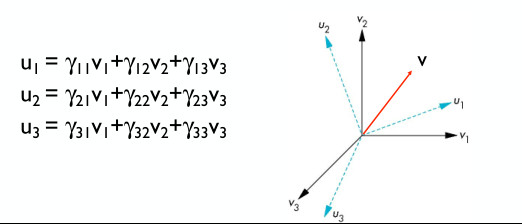
\includegraphics[scale=0.5]{pictures/basis.jpg}
		\end{center}
		\item Representing one Frame in Terms of the other:
		\begin{center}
			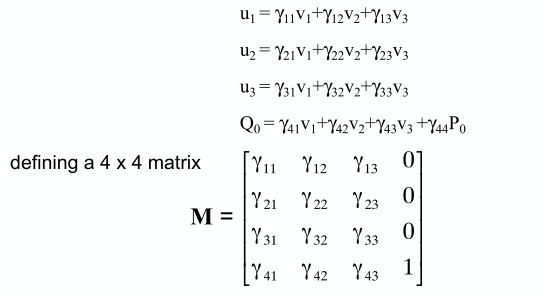
\includegraphics[scale=0.6]{pictures/framechange.jpg}
		\end{center}		
	\end{itemize}
	\subsection{Transformations}
	\begin{itemize}
		\item General Transformations: maps points/vectors to other points/vectors
		\item Translation: move of a point to a new location
		\begin{center}
			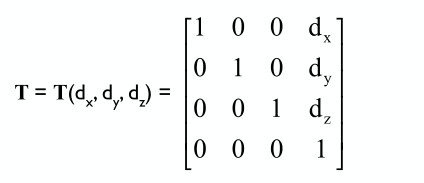
\includegraphics[scale=0.5]{pictures/translation.jpg}
		\end{center}
		\item Rotation: easy pattern you can learn if you know $x^{'} = x*\cos(\theta)-y\sin(\theta); x^{'} = x*\sin(\theta)+y\cos(\theta)$ and the rotation variable dosent change
		\begin{center}
			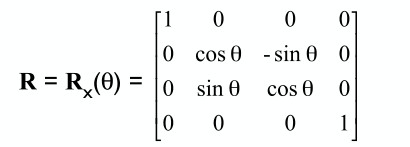
\includegraphics[scale=0.5]{pictures/rotationx.jpg}
			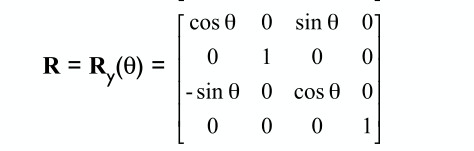
\includegraphics[scale=0.5]{pictures/rotationy.jpg}
			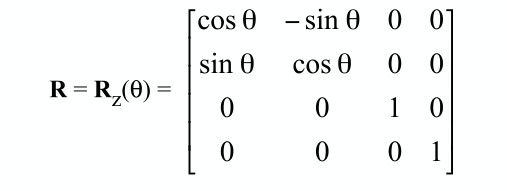
\includegraphics[scale=0.5]{pictures/rotationz.jpg}
		\end{center}
		\item Scaling: expand or contract along each axsis
		\begin{center}
			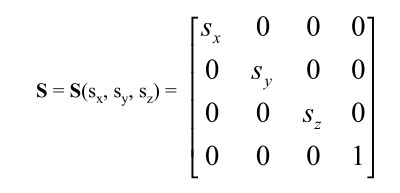
\includegraphics[scale=0.5]{pictures/scaling.jpg}
		\end{center}		
		\item Reflection: special case of Scaling, negative scaling variables
		\item Inverse: compute inverse matricies of tranformation matricies, using simple oberservation we can reduce this complex step
		\item Concatenation: if we use the same transformation for multiple verticies we can compute a overall transformation matrix using matrix multiplication and use this matrix on all vertices

	\end{itemize}
	\subsection{Homogeneous Coordinates}
	\subsection{Viewing}
	\subsection{Shading}

\section{Implementation}
	\subsection{Approaches (object vs image space)}
	\subsection{Implementing the pipeline}
	\subsection{Clipping}
	\subsection{Polygon Fill}
	
\section{Discrete Methods}
	\subsection{Buffers}
	\subsection{Bitmaps and Pixel Maps}
	\subsection{Texture Mapping}

\section{Programmmable Pipelines}
	\subsection{Shading Languages}
	\subsection{GLSL}
	\subsection{Vertex Shaders}
	\subsection{Fragment Shaders}

\section{Curves and Surfaces}
	\subsection{Representation of Curves and Surfaces}
	\subsection{Bézier Curves and Surfaces}
	\subsection{B-Splines}

\section{Advanced Rendering}
	\subsection{Radiosity}

\section{Hierarchies and Parallel Rendering}
	 \subsection{Traversal Methods}
	 \subsection{Scene Graphs}
	 \subsection{Parallel Rendering}

\end{document}

	